%
% Module 4 Chapter 7 Program Documentation
% CSC160-C00: Computer Science I (C++) (Jeffrey Hemmes)
% Author: Ashton Hellwig
% Date: 02 April 2020
%


\documentclass[a4paper, 11pt]{article}
  % Packages
  \usepackage[utf8]{inputenc}         % Encoding
  \usepackage[english]{babel}         % Internationalization
  \usepackage{times}                  % Times New Roman font
  \usepackage{soul}                   % Highlighting
  \usepackage{hyperref}               % Links (internal and external)
  \usepackage{fancyhdr}               % Headers and footers
  \usepackage[dvipsnames]{xcolor}     % Text Colors
  \usepackage{listings}               % Code Snippets
  \usepackage[section]{algorithm}     % For TOC support
  \usepackage{algpseudocode}          % Algorithmic notation environments
  \usepackage{enumitem}               % Ordered lists
  \usepackage{geometry}               % Page layout
  \usepackage{graphicx}               % Image support
  \usepackage{wrapfig}                % Sideways figures (landscape)
  \usepackage{lscape}                 % Sideways figures (landscape)
  \usepackage{rotating}               % Sideways figures (landscape)
  \usepackage{epstopdf}               % Sideways figures (landscape)
  \usepackage[toc, page]{appendix}    % Appendix
  \usepackage{setspace}               % Paragraph and line spacing
  \usepackage{bookmark}               % Required for appendix
  \usepackage{adjustbox}              % Required for appendix
  \usepackage{csquotes}               % Required for appendix
  \usepackage{amsthm}                 % Theorem environments
  \usepackage{array}                  % Arrays
  \usepackage{makecell}               % Table helpers
  \usepackage{amsmath}                % Mathematical symbols
  \usepackage[fleqn]{mathtools}       % Mathematical environments
  \usepackage{amssymb}                % Misc. symbols for logic and math
  \usepackage{relsize}                % Relative Sizing
  \usepackage{multicol}               % Multi-figure displays (grid)
  \usepackage{etoolbox,refcount}      % Required for mdframed
  \usepackage{parcolumns}             % Paragraph grids
  \usepackage{mdframed}               % Colored box environments
  \usepackage{float}                  % Floating Environments 
  \usepackage{aliascnt}               %
  \usepackage{multirow}               % Multiple rows in tables
  \usepackage[                        % Bibliography management
    backend=biber,%
    style=apa%
  ]{biblatex}

  % Bibliography Setup
  \addbibresource{main.bib}
  \DeclareBibliographyCategory{consulted}
  \addtocategory{consulted}{cpp:getline}
  % \newcommand{\CiteSection}[2]{%
    % (\autocite{#1}, ~\S {#1})%
  % }

%   \UseRawInputEncoding

  % Tables
  \renewcommand\theadalign{bc}
  \renewcommand\theadfont{\bfseries}
  \renewcommand\theadgape{\Gape[4pt]}
  \renewcommand\cellgape{\Gape[4pt]}

  % Lists
  \newcounter{countitems}
  \newcounter{nextitemizecount}
  \newcommand{\setupcountitems}{%
    \stepcounter{nextitemizecount}%
    \setcounter{countitems}{0}%
    \preto\item{\stepcounter{countitems}}%
  }
  \makeatletter
  \newcommand{\computecountitems}{%
    \edef\@currentlabel{\number\c@countitems}%
    \label{countitems@\number\numexpr\value{nextitemizecount}-1\relax}%
  }
  \newcommand{\nextitemizecount}{%
    \getrefnumber{countitems@\number\c@nextitemizecount}%
  }
  \newcommand{\previtemizecount}{%
    \getrefnumber{countitems@\number\numexpr\value{nextitemizecount}-1\relax}%
  }
  \makeatother
  \newenvironment{AutoMultiColItemize}{%
  \ifnumcomp{\nextitemizecount}{>}{3}{\begin{multicols}{2}}{}%
  \setupcountitems\begin{itemize}}%
  {\end{itemize}%
  \unskip\computecountitems\ifnumcomp{\previtemizecount}{>}{3}{\end{multicols}}{}}


  % Theorems
  \theoremstyle{definition}
  \newtheorem{defn*}{Definition}
  \theoremstyle{plain}
  \newtheorem{theorem*}{Equation}

  % Colors
  \newcommand{\commentstylecolor}{\color{Gray}}
  \newcommand{\keywordstylecolor}{\color{MidnightBlue}}
  \newcommand{\stringstylecolor}{\color{ForestGreen}}
  \newcommand{\questioninput}{\color{Red}}
  \newcommand{\answertcolor}{\color{Green}}
  \newcommand{\myanswer}{\answertcolor{\hl}}

  % Symbols
  \newcommand{\answerflow}{\rotatebox[origin=c]{180}{$\Lsh$}}
  \newcommand{\toanswer}{\mathlarger{\mathlarger{\answerflow}}\quad}

  % Math
  \newcommand{\highlight}[1]{%
    \colorbox{green!50}{$\displaystyle#1$}}

  % Image Directory
  \graphicspath{ {screenshots/} }


  % Hyperlink Setup
  \hypersetup{
    colorlinks = true,
    urlcolor = blue,
    linkcolor = blue
  }


  % Algorithm Settings
  \newcommand{\pluseq}{\mathrel{{+}{=}}}
  \newcommand{\minuseq}{\mathrel{{-}{=}}}


  % Syntax-Highlighting for Code Snippets
  \lstset{
    backgroundcolor=\color{white},
    breaklines=true,%
    captionpos=b,%
    frame=tlrb,%
    tabsize=2,%
    numbers=left,%
    showstringspaces=false,%
    commentstyle=\commentstylecolor,%
    keywordstyle=\keywordstylecolor,%
    stringstyle=\stringstylecolor%
  }
  \lstset{literate=
  {á}{{\'a}}1 {é}{{\'e}}1 {í}{{\'i}}1 {ó}{{\'o}}1 {ú}{{\'u}}1
  {Á}{{\'A}}1 {É}{{\'E}}1 {Í}{{\'I}}1 {Ó}{{\'O}}1 {Ú}{{\'U}}1
  {à}{{\`a}}1 {è}{{\`e}}1 {ì}{{\`i}}1 {ò}{{\`o}}1 {ù}{{\`u}}1
  {À}{{\`A}}1 {È}{{\'E}}1 {Ì}{{\`I}}1 {Ò}{{\`O}}1 {Ù}{{\`U}}1
  {ä}{{\"a}}1 {ë}{{\"e}}1 {ï}{{\"i}}1 {ö}{{\"o}}1 {ü}{{\"u}}1
  {Ä}{{\"A}}1 {Ë}{{\"E}}1 {Ï}{{\"I}}1 {Ö}{{\"O}}1 {Ü}{{\"U}}1
  {â}{{\^a}}1 {ê}{{\^e}}1 {î}{{\^i}}1 {ô}{{\^o}}1 {û}{{\^u}}1
  {Â}{{\^A}}1 {Ê}{{\^E}}1 {Î}{{\^I}}1 {Ô}{{\^O}}1 {Û}{{\^U}}1
  {œ}{{\oe}}1 {Œ}{{\OE}}1 {æ}{{\ae}}1 {Æ}{{\AE}}1 {ß}{{\ss}}1
  {ű}{{\H{u}}}1 {Ű}{{\H{U}}}1 {ő}{{\H{o}}}1 {Ő}{{\H{O}}}1
  {ç}{{\c c}}1 {Ç}{{\c C}}1 {ø}{{\o}}1 {å}{{\r a}}1 {Å}{{\r A}}1
  {€}{{\euro}}1 {£}{{\pounds}}1 {«}{{\guillemotleft}}1
  {»}{{\guillemotright}}1 {ñ}{{\~n}}1 {Ñ}{{\~N}}1 {¿}{{?`}}1
}
  \newenvironment{alltt}{\ttfamily}{\par}
  \lstMakeShortInline[language=c++,columns=fixed]|

  % Page Configuration
  %% Style
  \pagestyle{fancy}

  %% Layout
  \geometry{%
    a4paper,%
    top=2.5cm,%
    bottom=2.5cm,%
    left=2.5cm,%
    right=2.5cm%
  }
  %%% Document
  \setlength{\headheight}{15pt}
  \setlength{\floatsep}{12pt}
  \setlength{\parindent}{2em}
  \setlength{\parskip}{0.5em}
  \renewcommand{\baselinestretch}{.9}

  %% Title page
  \title{Chapter 7 Programming Assignment Documentation}
  \author{Ashton Hellwig}
  \date\today
  \setcounter{tocdepth}{3}

  %% Subsequent pages
  \lhead{CSC160}
  \rhead{Computer Science I (C++)}
  \lfoot{M4C7Program}
  \rfoot{A. Hellwig}


  % Document Content
\begin{document}
  % Title Page
  \maketitle
  \tableofcontents
  \listofalgorithms
  \lstlistoflistings
  \listoffigures
  \newpage


  % Problem Analysis
  \section{Problem Analysis}
    The problem states:
    \begin{mdframed}[backgroundcolor=green!20]
      This assignment relates to content from Chapter 7 of the eText.

      \textbf{Instructions}\vspace{-8pt}
      \begin{enumerate}
        \item Review the general programming assignment instructions.
        \item Write a program that reads in a line consisting of a student`s
          name (first and last), Social Security number, user ID, and password.
          \begin{itemize}
            \item Use |std::getline()| not |std::cin| so you can demonstrate an
              understanding of the string manipulation concepts. For an example
              of how getline works see example code
              \href{http://www.cplusplus.com/reference/string/string/getline}%
              {here}.
          \end{itemize}
        \item The program outputs the string in which all the digits of the
          Social Security number and all the characters in the password are
          replaced by x.
          \begin{itemize}
            \item The Social Security number is in the form 000-00-0000, and the
              user ID and the password do not contain any spaces.
          \end{itemize}
        \item Your program should not use the operator [] to access a string
          element. Use the appropriate functions described in Table 7-1 of the
          textbook.
      \end{enumerate}
    \end{mdframed}

    \subsection{Data}
      \begin{itemize}
        \item We should be using the functions described in \S~7-3a, Table 7-1
          in order to access the string element (See Appendix
          \ref{app:stringfuncs})
        \item User ID and password contain no spaces.
        \item Social security number is an |std::string| in the format of
          \texttt{000-00-0000}.
      \end{itemize}

    \subsection{Desired Output}
      \begin{lstlisting}[%
        language=bash,%
        columns=flexible,%
        caption={ashellwig\_m4c7\_programming\_assignment output %
          (stdout)},%
        label={desiredoutput:stdout}%
    ]
Enter a student's name, social security number, user id, and password
in one line:
Jane Smith 22-33-4444 S12345 password

Jane Smith xx-xx-xxxx S12345 xxxxxxxx
Press any key to continue...
      \end{lstlisting}


  % Algorithm
  \newpage
  \section{Algorithm}
    Below is the algorithm for the program.
    \begin{algorithm}[H]
      \caption{Chapter 7 Program Algorithm}
      \vspace{12pt}
      \begin{algorithmic}[1]
        \Function{obscureData}{$inputData$}
          \State $outputData\gets\ inputData$
          \State $position\gets\ 0$
          \State
          \While{$true$}
            \State $firstSpace\gets\ $\Call{findChar}{$\text{`` ''}$}
              \Comment{First space in string should be before last name}
            \State $position\gets\ $
              \Call{findChar}{$\text{`` ''}$, $firstSpace+1$} $+1$
              \Comment{After the second space is our SSN}
            \State\State
              $($\Call{replace}{$position, \text{xxx-xx-xxxx}$}$)*11$
              \Comment{Replace the next 11 characters}
            \State $position\pluseq 10$
              \Comment{%
                Advance position so we don`t replace the same substring again%
              }
            \State\Comment{Skip the next two spaces so we hit our password}
            \State $position\gets $\Call{findChar}{$\text{`` ''}$, $position+1$}
            \State $position\gets $\Call{findChar}{$\text{`` ''}$, $position+1$}
            \State\State
            \State $position\pluseq 1$\Comment{Replace the next char, not space}
            \While{$position\ <\ $ \Call{lengthOf}{outputData}}
              \Comment{Replace the characters from pos$\rightarrow$end}
              \State
                \Call{replace}{$position, \text{x}$}
                \State $positon\pluseq 1$
              \State
              \If{$position =\ $\Call{lengthOf}{outputData}}
                \State\Call{exitLoop}{}
              \EndIf
            \EndWhile
          \EndWhile
          \State\State
          \Return $outputData$
            \Comment{Return our modified string}
        \EndFunction
        \State
        \Procedure{main}{}
          \State $studentData\gets\ \text{``\textbackslash0x''}$
          \State\State
            \Call{toOutput}{``Enter a student's name, social security number,
              user id, and password in one line:''}
          \State\State
            \Call{setFromIO}{$stdin$,$studentData$}
          \State
          \State $outData\gets\ $\Call{obscureData}{$studentData$}
          \State\State
            \Call{toOutput}{$outData$}
        \EndProcedure
      \end{algorithmic}
      \label{alg}
    \end{algorithm}


  % User Documentation
  \newpage
  \section{User Documentation}
    Please see Appendix \ref{appendix:img} for images showing the compilation
      and running of the program.

    %% Usage
    \subsection{Build}
      The following are instructions with two use cases:
      \begin{itemize}
        \item With GNU Make
        \item Bundled Release
      \end{itemize}
      \subsubsection{With GNU Make}
        \begin{enumerate}
          \item Navigate to the unzipped folder containing the project,
            \textbf{with a terminal emulator or command prompt}, this will
            (most likely) mean running:
            \begin{lstlisting}[language=bash]
cd ~/Downloads/ashellwig_m4c7_programming_assignment
            \end{lstlisting}
          \item Compile the program and documentation\footnote{\textbf{Note%
            }: This requires the whole \texttt{texlive} suite as well as
            \texttt{latexmk} to be installed.} using GNU automake after
            switching to the source directory:
            \begin{lstlisting}[%
              language=bash,%
              caption={Chapter 7 Program Build Commands},%
            ]
make debug

./out/bin/ashellwig_m4c7_programming_assignment.bin # Run program

make clean-all # Removes object files, binaries, and docs
            \end{lstlisting}
          \end{enumerate}
      \subsubsection{Bundled Release}
        \begin{enumerate}
          \item Navigate to the unzipped folder containing the binary,
            \textbf{with a terminal emulator or command prompt}, this will
            (most likely) mean running:
            \begin{lstlisting}[language=bash]
cd ~/Downloads/ashellwig_m4c7_programming_assignment/out/bin
            \end{lstlisting}
          \item To run the program simply issue this within the command
            prompt
            \begin{lstlisting}[language=bash]
./build/ashellwig_m4c7_programming_assignment
            \end{lstlisting}
        \end{enumerate}
        Of course if preferred, you may also navigate to the build folder in
          file explorer and double click the executable
          (\texttt{./ashellwig\_m4c7\_programming\_assignment}).


  % Bibliography
  \newpage
  \nocite{*}
  \printbibliography[%
    heading=bibintoc,%
    title={Works Cited},%
    notcategory={consulted}%
  ]{}
  \printbibliography[%
    heading=bibintoc,%
    title={Works Consulted},%
    category={consulted}%
  ]{}

  % Appendix
  \appendix
  \newpage
  % Images
  \section{Images}\label{appendix:img}
    \begin{figure}[H]
      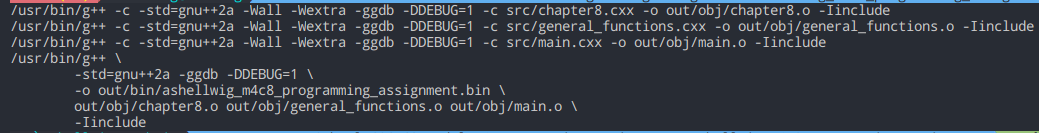
\includegraphics[%
        width={\textwidth}%
      ]{compile.png}
      \caption{Compiling Chapter 7`s Program}
      \label{img:compilation}
    \end{figure}
    \begin{figure}[H]
      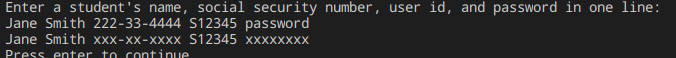
\includegraphics[%
        width=\textwidth%
      ]{run.png}
      \caption{Running Chapter 7`s Program}
      \label{img:running}
    \end{figure}


  \newpage
  \section{Unit Tests}
    Tests were written with the
      \href{https://github.com/catchorg/catch}{Catch2 library}. The output is
      shown below.

    \begin{figure}[H]
      \caption{Test Output}
      \centering
      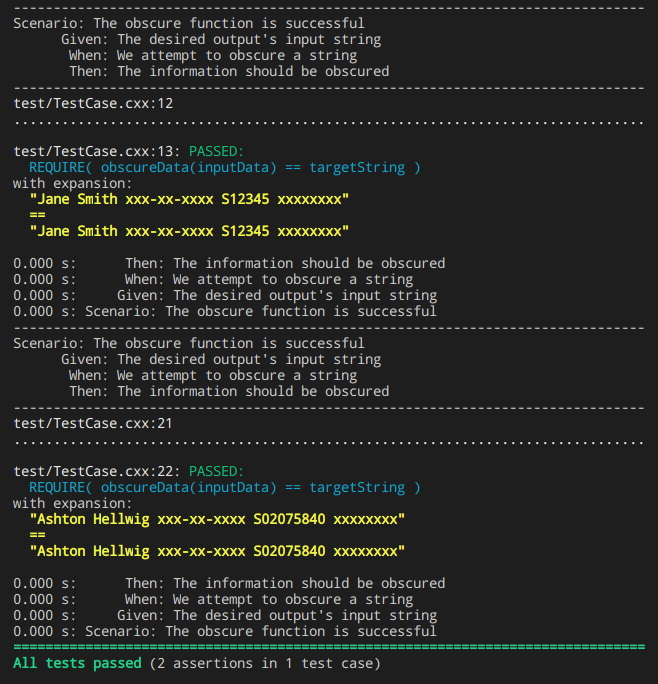
\includegraphics[width=\textwidth]{testout.png}
    \end{figure}

    \newpage
    \subsection{Unit Test File}
      Below I have included the code used to run the unit test for reference.

      \begin{lstlisting}[language=c++,caption={TestCase.cxx}]
#include "../include/catch2/catch.hpp"
#include "./include/test_helpers.hh"
#include <sstream>
#include <string>

SCENARIO("The obscure function is successful", "[functions]") {
  GIVEN("The desired output's input string") {
    WHEN("We attempt to obscure a string") {
      std::string inputData = "Jane Smith 222-33-4444 S12345 password";
      std::string targetString = "Jane Smith xxx-xx-xxxx S12345 xxxxxxxx";

      THEN("The information should be obscured") {
        REQUIRE(obscureData(inputData) == targetString);
      }
    }
    WHEN("We attempt to obscure a string") {
      std::string inputData = "Ashton Hellwig 111-11-1111 S02075840 password";
      std::string targetString =
          "Ashton Hellwig xxx-xx-xxxx S02075840 xxxxxxxx";

      THEN("The information should be obscured") {
        REQUIRE(obscureData(inputData) == targetString);
      }
    }
  }
}
      \end{lstlisting}

    \newpage
    \section{String Functions}\label{app:stringfuncs}
      The following functions should be used rather than the [] operator
        to access string elements, taken from \S~7-3a Table 7-1
        \parencite[\S~7-3a]{textbook}.

      \begin{figure}[H]
        \centering
        \caption{Textbook Table 7-1}
        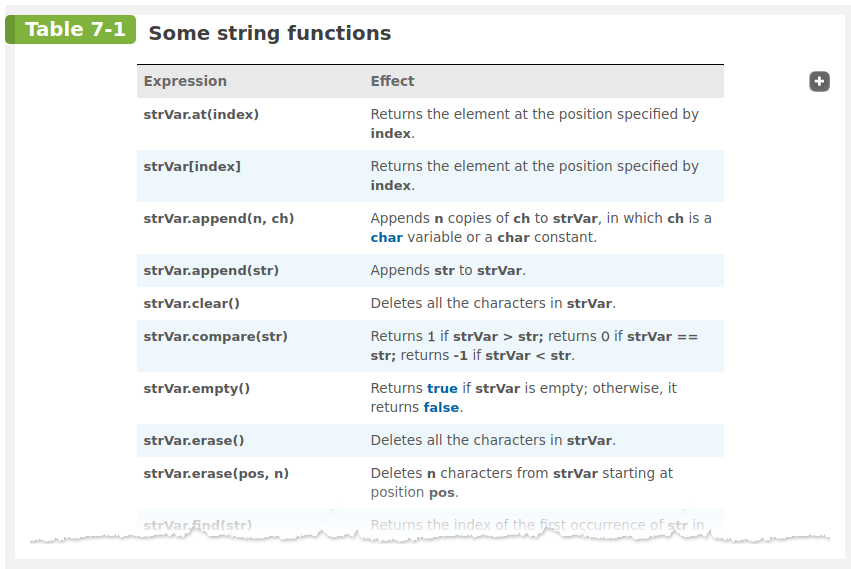
\includegraphics[width=\textwidth]{stringfuncs.png}
      \end{figure}
      \newpage
      \begin{figure}[H]
        \centering
        \caption{Textbook Table 7-1 (Pt 2)}
        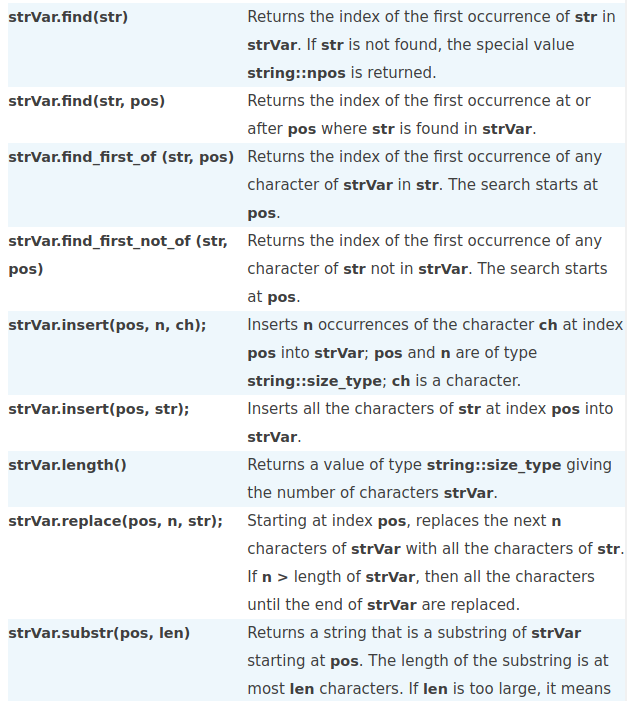
\includegraphics[width=\textwidth]{stringfuncs2.png}
      \end{figure}
      \newpage
      \begin{figure}[H]
        \centering
        \caption{Textbook Table 7-1 (Pt 2)}
        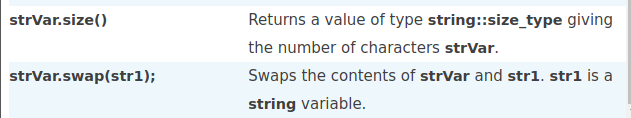
\includegraphics[width=\textwidth]{stringfuncs3.png}
      \end{figure}
\end{document}

